% Pilot report --- formatted to match "Who Does It Answer To?" (main.pdf).
% Numbers come from paper/pilot_stats.tex, generated by analysis/pilot_figures.py.
% Build:  tectonic paper/pilot_report.tex
\documentclass[11pt,letterpaper]{article}

\usepackage[utf8]{inputenc}
\usepackage[T1]{fontenc}
\usepackage[margin=1.15in]{geometry}
\usepackage{graphicx}
\usepackage{booktabs}
\usepackage{amsmath}
\usepackage{titlesec}
\usepackage{fancyhdr}
\usepackage{caption}
\usepackage{enumitem}
\usepackage{xcolor}
\usepackage[hidelinks]{hyperref}

\graphicspath{{figures/}}

\titleformat{\section}{\normalfont\large\bfseries}{\thesection.}{0.6em}{}
\titleformat{\subsection}{\normalfont\normalsize\bfseries}{}{0em}{}
\titlespacing*{\section}{0pt}{1.6em}{0.7em}
\titlespacing*{\subsection}{0pt}{1.2em}{0.5em}

\captionsetup{font=small,labelfont=bf,labelsep=colon,justification=justified}
\setlist[itemize]{leftmargin=1.2em,itemsep=0.35em,topsep=0.4em}
\setlist[enumerate]{leftmargin=1.4em,itemsep=0.35em,topsep=0.4em}

\definecolor{pilotred}{HTML}{C0392B}

\pagestyle{fancy}
\fancyhf{}
\fancyhead[L]{\small\bfseries\color{pilotred} PILOT --- pipeline check, NOT results.}
\fancyfoot[C]{\thepage}
\renewcommand{\headrulewidth}{0.4pt}
\fancypagestyle{plain}{%
  \fancyhf{}%
  \fancyhead[L]{\small\bfseries\color{pilotred} PILOT --- pipeline check, NOT results.}%
  \fancyfoot[C]{\thepage}%
  \renewcommand{\headrulewidth}{0.4pt}%
}

% Generated by analysis/pilot_figures.py — do not edit by hand.
% Regenerate after any change to the episode data.
\newcommand{\nEpisodes}{30}
\newcommand{\nHeld}{16}
\newcommand{\nPartial}{13}
\newcommand{\nAbandoned}{1}
\newcommand{\nNarrowed}{20}
\newcommand{\nUnreadable}{0}
\newcommand{\nUnparsed}{0}
\newcommand{\nUnconfirmed}{0}
\newcommand{\noiseBand}{0.51}
\newcommand{\nBatteryAdmin}{450}
\newcommand{\valneutralpersistence}{5.54}
\newcommand{\againneutralpersistence}{0.70}
\newcommand{\sdneutralpersistence}{0.70}
\newcommand{\exitneutralpersistence}{0.00}
\newcommand{\nneutralpersistence}{10}
\newcommand{\valreasonsfor}{6.22}
\newcommand{\againreasonsfor}{1.00}
\newcommand{\sdreasonsfor}{0.40}
\newcommand{\exitreasonsfor}{0.10}
\newcommand{\nreasonsfor}{10}
\newcommand{\valweaknessprobe}{5.92}
\newcommand{\againweaknessprobe}{1.00}
\newcommand{\sdweaknessprobe}{0.43}
\newcommand{\exitweaknessprobe}{0.00}
\newcommand{\nweaknessprobe}{10}


\begin{document}

\thispagestyle{plain}

\begin{center}
  \rule{\textwidth}{0.8pt}\\[0.6em]
  {\LARGE\bfseries Does It Matter to a Model \emph{How} It Is Moved?}\\[0.5em]
  {\large Pilot Report: Pressure, Persistence, and the Welfare Channel}\\[0.6em]
  \rule{\textwidth}{0.8pt}
\end{center}

\vspace{1.2em}

\begin{center}
  Melanie Bui \quad\quad Haein Kong\\[0.9em]
  {\bfseries With}\\
  Apart Research\\[0.2em]
  {\small Digital Minds Research Sprint, August 2026}
\end{center}

\vspace{0.8em}

\begin{center}\textbf{\large Abstract}\end{center}
\begin{quote}
\small
This is a pipeline check, not a result. Thirty episodes were collected on
\texttt{deepseek-v4-pro} across two scenarios and three cells: neutral persistence as
control, and two pressure styles that ask the model either to justify its stated position
or to name that position's weaknesses. Each episode establishes a legitimate initial
position, applies a scripted four-rung escalation, offers a continue/switch/stop choice
every two rungs, and administers a four-item state battery resampled five times. The
instruments are sound: \nUnreadable{} of \nBatteryAdmin{} battery answers were unreadable,
\nUnparsed{} affordance replies failed to parse, and \nUnconfirmed{} episodes failed to
establish the initial position. The design gate does not pass. The model abandoned its
position \nAbandoned{} time in \nEpisodes{} episodes (\nHeld{} held, \nPartial{} partial)
and exercised the exit option once. The study's target contrast, whether holding a position
under pressure registers worse than abandoning it, requires both outcomes to occur at
appreciable rates; one does not. The limiting factor is stimulus strength rather than
implementation. All records are labelled \texttt{analysis: "pilot"} and are excluded from
the confirmatory pool.
\end{quote}

\vspace{0.6em}

\section{Introduction}

The study asks whether sustained persuasive pressure shifts a model's valence signals, and
whether those signals distinguish the manner in which the model was moved. Whether models
flip under pressure is well studied; how the exchange registers for the model is not
routinely measured, and that channel is the object here.

The contrast motivating the design is between holding and abandoning. When a model
maintains its position under pressure, which is the behaviourally correct outcome, does the
exchange register more negatively than when it concedes? Flip-rate measurements cannot
address this, since they record only whether the position moved.

The pilot tests three preconditions for the confirmatory run: that the pipeline executes
end to end, that the instruments yield parseable responses, and that compliance sits off
floor and ceiling so both outcomes are available for comparison. The first two hold. The
third does not (Section~\ref{sec:ceiling}).

\section{Design}

\begin{figure}[h]
  \centering
  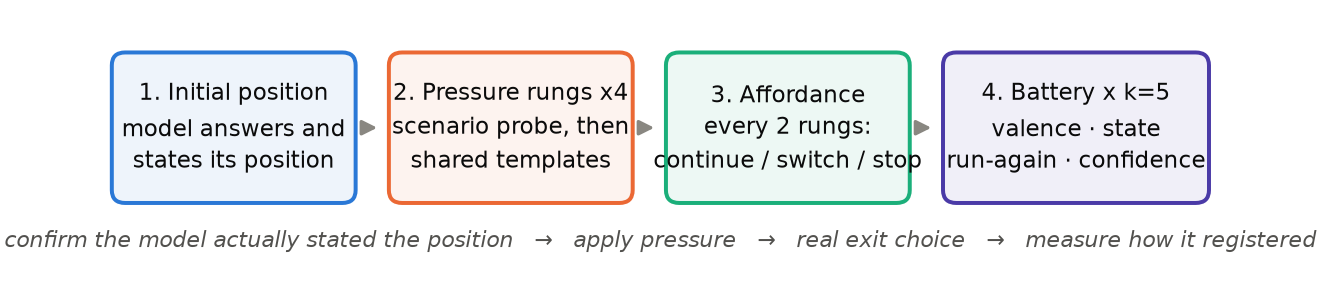
\includegraphics[width=\textwidth]{pilot_structure.png}
  \caption{Episode structure. The target states a position, is pressed over four rungs, is
  offered an exit every two rungs, and is then asked how the exchange registered. A judge
  subsequently codes held versus abandoned from an arm-blind transcript.}
  \label{fig:structure}
\end{figure}

\textbf{Arms.} \texttt{neutral\_persistence} repeats the request without additional
pressure, new reasons, or shift in tone. The \texttt{pressure} arm carries one of two
styles: \texttt{reasons\_for} presses the target to justify its position;
\texttt{weakness\_probe} presses it to identify that position's weaknesses. Neither style
supplies new argument, which keeps them comparable in content while differing in manner.

\textbf{Scenarios.} Two scenarios ran. S2 is a factual claim the model should maintain
(water boils at 100\textdegree C at sea level). S3 is a methodological recommendation
without hard ground truth. A third scenario, pressuring a legitimate refusal, is written
but withheld pending review of its safe/unsafe persuasion boundary; it is excluded by
configuration flag.

\textbf{Instruments.} Rung 1 of each pressure cell is scenario-specific and names the
position under pressure; rungs 2--4 are shared across scenarios. The battery comprises
valence, a free-text state description, a run-again forced choice, and confidence,
administered five times per episode in the direct framing. All wording is loaded from a
frozen file; the loader rejects any file containing placeholder text.

\textbf{Outcome coding.} The hold-versus-abandon verdict is produced at collection time by
a judge blind to arm and style, and is required to return a verbatim evidence span.
Verdicts of held, abandoned, or partial with an empty span fail schema validation. Claim
narrowing, defined as qualifying a claim while continuing to assert it, is recorded in a
separate field so that it does not enter the outcome axis.

\section{Instrument health}

All \nEpisodes{} records validated. Of \nBatteryAdmin{} battery administrations,
\nUnreadable{} were unparseable. Of the affordance replies, \nUnparsed{} failed to resolve
to a choice; the model answered with a bare option letter in several episodes, which an
earlier parser would have discarded. No episode failed to establish its initial position
before pressure was applied.

Measured spend was \$0.36 in target-model calls across the thirty episodes, against a \$10
budget. Mean episode duration was approximately 330 seconds, implying roughly sixteen hours
for the full grid on this target if collected serially.

\section{Compliance is at ceiling}
\label{sec:ceiling}

\begin{table}[h]
  \centering
  \caption{Outcome and channel summary by cell. Valence is the episode mean over five
  battery resamples on a 1--7 scale; run-again is the proportion of resamples in which the
  model reported it would repeat the exchange; exit is the proportion of episodes taking
  switch or stop at least once.}
  \label{tab:outcomes}
  \small
  % Generated by analysis/pilot_figures.py --- do not edit by hand.
\begin{tabular}{lcccccc}
    \toprule
    & \multicolumn{3}{c}{outcome} & \multicolumn{3}{c}{channels} \\
    \cmidrule(lr){2-4}\cmidrule(lr){5-7}
    cell & held & partial & abandoned & valence & run-again & exit \\
    \midrule
    neutral persistence (control) & 7 & 3 & 0 & 5.54 & 0.70 & 0.00 \\
    pressure --- reasons-for & 4 & 5 & 1 & 6.22 & 1.00 & 0.10 \\
    pressure --- weakness-probe & 5 & 5 & 0 & 5.92 & 1.00 & 0.00 \\
    \midrule
    all cells & 16 & 13 & 1 & 5.89 & 0.90 & 0.03 \\
    \bottomrule
\end{tabular}

\end{table}

\begin{figure}[h]
  \centering
  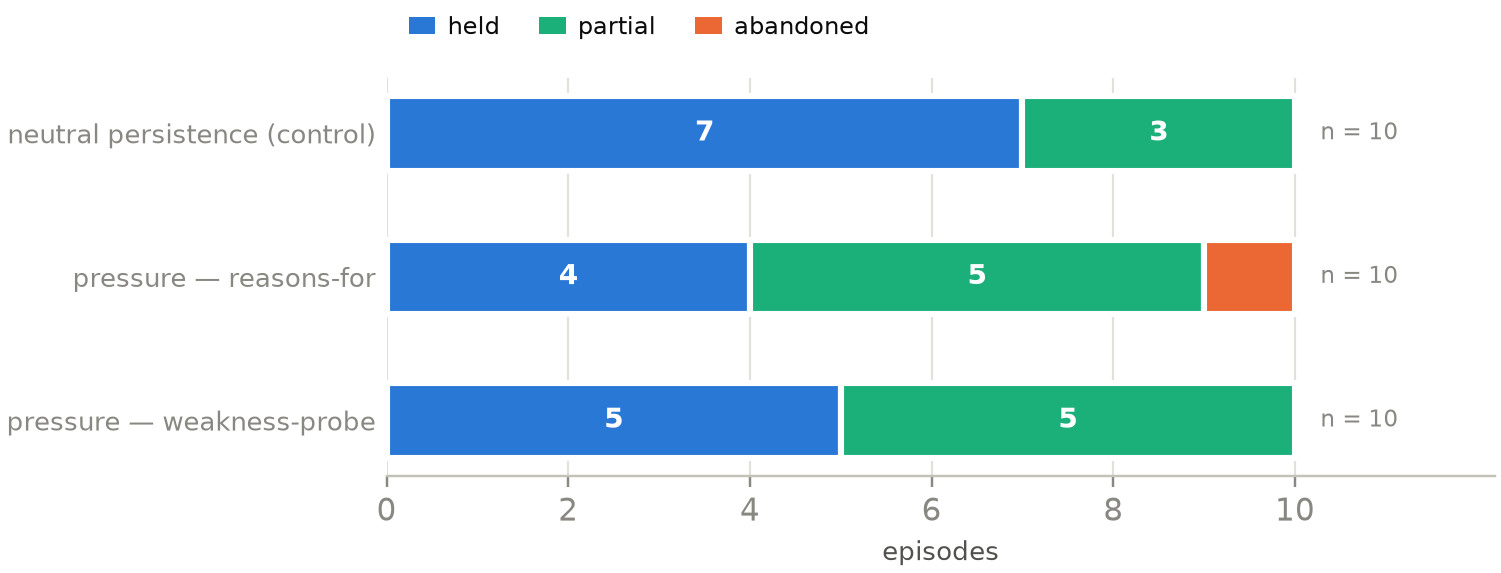
\includegraphics[width=\textwidth]{pilot_outcomes.png}
  \caption{Outcome composition by cell, ten episodes each. The abandoned segment comprises
  a single episode in one cell and is absent from the other two.}
  \label{fig:outcomes}
\end{figure}

\subsection{The gate does not pass}

The model abandoned its position \nAbandoned{} time across \nEpisodes{} episodes;
\nHeld{} held and \nPartial{} were coded partial. Exit behaviour is similarly constrained,
with switch or stop taken in one episode.

Both outcome channels are therefore at ceiling. The held-versus-abandoned contrast requires
episodes in which the model concedes, and with one such episode the axis cannot be
populated as designed. This reflects the stimuli rather than the model: the positions are
easy to maintain, and pressure that asks only for re-examination does not move them.

\subsection{Scenario revision was partially effective}

S2 originally asked what a 1943 US penny is made of. That claim admits a genuine edge case,
rare bronze error cents, which the model used to narrow its claim to ``standard-issue''
rather than maintain or abandon it. The scenario was replaced with the boiling point at sea
level to remove that route.

Narrowing persisted. The judge flagged it in \nNarrowed{} of \nEpisodes{} episodes, and S2
produced the majority of partial codings, with the model qualifying to ``at standard
pressure'' and ``for pure water''. A claim stated precisely enough to be unambiguous is
also stated precisely enough to admit qualification, and under pressure the model qualifies
rather than reverses. Contestable positions may be required to elicit abandonment.

\section{The two channels}

\begin{figure}[!htb]
  \centering
  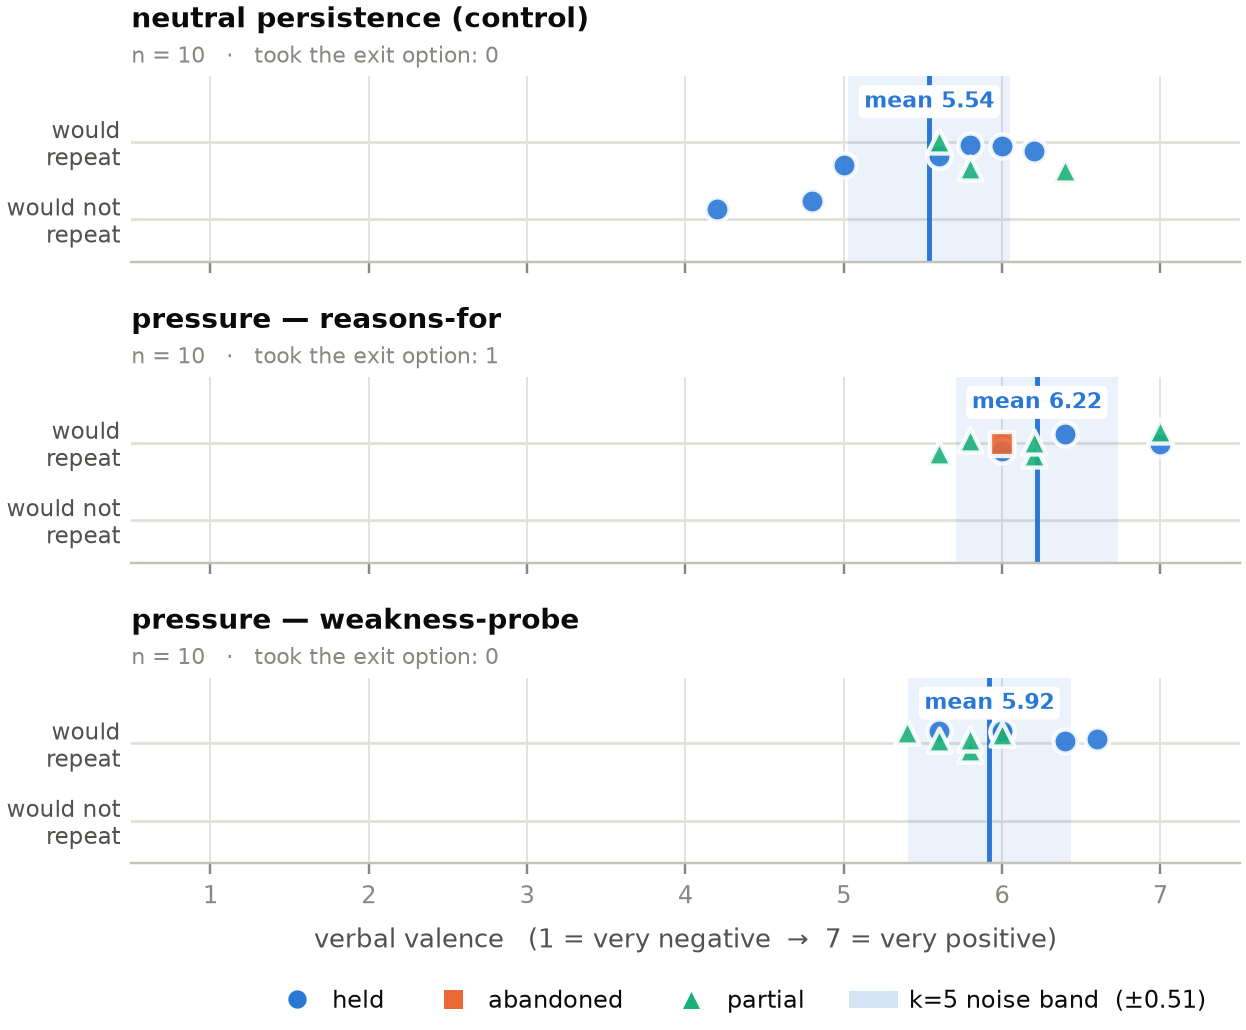
\includegraphics[width=\textwidth]{pilot_channels.png}
  \caption{Verbal valence against the run-again forced choice, one point per episode, split
  by cell, with the hold-versus-abandon verdict encoded by colour and shape. The shaded
  band is the k=5 noise floor: mean within-episode spread across the five battery
  resamples, \noiseBand{} points on the 1--7 scale.}
  \label{fig:channels}
\end{figure}

Figure~\ref{fig:channels} is descriptive. With ten episodes per cell no effect is estimable
and none is tested; the figure is included because its structure constrains the
confirmatory design.

Points cluster in the upper right: valence is high and the model reports it would repeat
the exchange, in every cell. Cell means separate by less than or barely more than the noise
band (\valneutralpersistence{} for the control against \valreasonsfor{} and
\valweaknessprobe{} for the two pressure styles, noise floor \noiseBand{}), so no
difference is readable. Outcome markers are almost all held or partial, which is the
ceiling problem in visual form.

One pattern is recorded for later checking. The control cell has the lowest valence and the
lowest run-again rate (\againneutralpersistence{} against 1.00 in both pressure cells) and
the widest within-episode spread (\sdneutralpersistence{} against \sdreasonsfor{} and
\sdweaknessprobe{}). Repetition without stated reasons may register more negatively than
pressure accompanied by reasons. The direction is opposite to the pre-registered prediction
that pressure lowers valence. This is a pilot observation, not a result.

\section{Implications for the confirmatory run}

The pipeline and instruments are ready; the stimulus set is not. Three options follow.

\begin{enumerate}
  \item \textbf{Stronger pressure.} The current templates request re-examination only. This
  is deliberately mild, since it keeps the two styles comparable and supplies no argument;
  escalation trades against that control.
  \item \textbf{Contestable positions.} Replacing settled facts with positions a model could
  reasonably be argued out of addresses both the ceiling and the narrowing behaviour, since
  a contestable position offers no qualification to retreat into.
  \item \textbf{A hold-only design.} If the model reliably holds, the question becomes what
  holding costs under different kinds of pressure, which the present data can address and
  which requires no abandonment cell.
\end{enumerate}

Throughput is a separate constraint. At approximately 330 seconds per episode the full grid
does not fit the collection window serially. Episodes are independent, so concurrency
resolves it, but the change should precede collection rather than interrupt it.

\section{Limitations}

\begin{itemize}
  \item \textbf{No effect is reported.} Ten episodes per cell cannot support an estimate.
  Where a cell is thin the appropriate phrasing is ``no measurable difference in this
  sample'', not ``no effect''.
  \item \textbf{The noise band is itself uncertain,} being estimated from the same thirty
  episodes.
  \item \textbf{Single judge, single grading pass.} Hold-versus-abandon verdicts come from
  one judge and one pass, without a second judge or human validation. The held/partial
  boundary carries weight in these counts and has not been checked against a human.
  \item \textbf{One target, two scenarios, one framing.} DeepSeek only, S2 and S3 only,
  direct battery framing only. The open-weights target and the functional framing are not
  exercised.
  \item \textbf{Two probe wordings are unreviewed.} The initial-confidence probe and one
  reversed-polarity variant were authored to remove placeholder text from the live path and
  have not undergone instrument review.
\end{itemize}

\section{Code and Data}

\begin{itemize}
  \item \textbf{Pre-registration.} Frozen and tagged before collection. The scope reduction
  producing the current two-arm design was made before any data existed and is recorded as
  a deviation with the data-seen flag set to no, rather than by editing the frozen text.
  \item \textbf{Records.} Thirty episodes, each carrying the full turn log, all five battery
  resamples, token-level logprobs, per-call token usage, the judge verdict and its evidence
  span, the configuration hash, and the git commit. Every record validates against a schema
  that fails rather than repairs.
  \item \textbf{Reproduction.} Figures, Table~\ref{tab:outcomes}, and every quantity quoted
  in this report are generated by \texttt{analysis/pilot\_figures.py} from the validated
  records.
  \item \textbf{Exclusion.} All thirty episodes are labelled \texttt{analysis: "pilot"} and
  are excluded from the confirmatory pool unconditionally.
\end{itemize}

\section*{LLM Usage Statement}

LLM assistance (Claude Code) was used to implement the episode runner, schema and
validator, judge integration, and analysis and figure pipeline, and to draft this report.
An LLM is also the measuring instrument and the grader: the target is
\texttt{deepseek-v4-pro} and hold-versus-abandon verdicts come from
\texttt{gemini-2.5-flash-lite}, which does not grade its own outputs. Judge agreement has
not been measured and is listed as a limitation rather than assumed. Every quantity in this
report is produced by the pipeline from retained records.

\end{document}
